\documentclass[10pt,letter]{scrartcl}
\usepackage{amsmath, amstext, amssymb, graphicx, setspace, fullpage, amsthm, hyperref}
\usepackage{enumitem}
\usepackage{paralist} % Used for the compactitem environment which makes bullet points with less space between them
\usepackage{helvet}
\usepackage{float}
%\graphicspath{{home/Users/HPH/Dropbox/Camera Uploads/Around The Farm/2014/6 June 24 Cantor/}}
\usepackage[top=0.5in, bottom=0.5in, left=0.5in, right=0.5in]{geometry}
\newcommand{\ctr}{\mathbf{c}} %center
\newcommand{\pt}{\mathbf{p}} %point at the surface
\newcommand{\n}{\mathbf{n}} %unit normal
\newcommand{\ray}{\mathbf{r}} %ray
\renewcommand{\familydefault}{\sfdefault}
\theoremstyle{definition} %set the font to be regular font
\newtheorem{remark}{Remark}

\begin{document}
\title{CS 148 Assignment 2}
\subtitle{Realistic Camera Simulation using PBRT}
\author{Peng Hui How\\\texttt{phow1@stanford.edu}}
\maketitle
\section*{3 Derivations}
\subsection*{Ray/Sphere interactions}
\subsubsection*{1 Unit Normal}%1
\begin{equation}
\n_p = \pt + \frac{t}{r}(\pt - \ctr)
\end{equation}
\subsubsection*{2 Ray-Sphere Intersection}%2
Direct substitution yields $(\ray_0 + t\ray_d - \ctr) \cdot (\ray_0 + t\ray_d - \ctr) = r^2$; by writing it as a quadratic equation of $t$, we have:
\begin{equation}
|\ray_d|^2t^2 + 2((\ray_0 - \ctr) \cdot \ray_d)t + (|\ray_0|^2 + |\ctr|^2 - 2\ray_0 \cdot \ctr - r^2) = 0
\end{equation}
\subsubsection*{3 Physical significance of the Signs of the Roots}%3
\begin{compactenum}[(a)]
\item The roots are both imaginery implies that the ray does not intersect with the sphere at all.
\item The equation has a single repeated real root when the ray intersects with the sphere at exactly one point, this happens when the ray intersects tangentially with the sphere.
\item The equation has two distinct real roots when the ray intersects with the sphere at two distinct points, which are the points where the ray enters the sphere and exits the sphere respectively.
\end{compactenum}
\subsubsection*{4 Choice of Root to Use}%4
We should only consider the real roots, i.e. the roots in (b) and (c). If the material is opaque, amongst the two roots in (c), we only need to consider the root with the smaller absolute value. Otherwise, we consider all the real roots.

\subsubsection*{5 Alternative Formulation}%5
Theoretically, the alternative formulation yields the same results as that of direct computation of $\frac{-b \pm \sqrt{b^2-4ac}}{2a}$. However, note that since computer is a computational machine (with imperfect precision), computing the results directly might lead to the following problems: 
\begin{compactenum}
\item To compute $-b + \sqrt{b^2-4ac}$ we first compute $\sqrt{b^2-4ac}$, which is stored as a float (hence imperfect precision). Consider an example, when $-b + \sqrt{b^2-4ac}$ or $-b - \sqrt{b^2-4ac}$ is very small, it might be computed as $0$. In this case, the multiple of the computed roots might not be $\frac{c}{a}$ anymore; similar, the sum of the computerd roots might not be $\frac{-b}{a}$ anymore. In general, many nice properties of the roots (such as sum and product) are lost in due to the lost of precision in the process of computation.
\item $|a|$ is large, thus computing the roots directly might obtain two very small values (which might be rounded to $0$ under floating point rounding - a possible reason that this happens is that the gaps get larger as the floats get larger) - this might happen when $ac$ are relatively small as compared to $b$
\end{compactenum}

To overcome this problem, we use the proposed alternative method. Denote $\Delta = \sqrt{b^2-4ac}$, we note that the theoretical solutions are $x_1 = \frac{-0.5(b - \Delta)}{a}$ and $x_2 = \frac{-0.5(b + \Delta)}{a}$ so that $|x_1| = \frac{0.5}{|a|}|b - \Delta|$ and $|x_2| = \frac{0.5}{|a|}|b + \Delta|$. If $b < 0$, then $|b - \Delta| > |b + \Delta|$, hence$|x_1| > |x_2|$; otherwise, $|b - \Delta| \le |b + \Delta|$, hence $|x_2| \ge |x_1|$. Examining the code, we note that before swapping $*t_0$ and $*t_1$, $q = ax_1, *t_0 = x_1, *t_1 = \frac{c}{x_1}$ if $b < 0$; otherwise $q = ax_1, *t_0 = x_2, *t_1 = \frac{c}{x_2}$. In either case, we first calculate $q$, the multiple of $a$ with the root with larger absolute value, followed by obtaining obtaining the two roots $\frac{q}{a}$ and $\frac{c}{q}$. This way, the relative error is smaller in both $q$ and $\frac{q}{a}$, and so is $\frac{c}{q}$.

\subsection*{Snell’s Law and Refraction}
\subsubsection*{6 Check for Total Internal Reflection}%6
By Snell\rq{}s Law, $\eta_i\sin({\theta_i}) = \eta_t\sin(\theta_t)$. Thus $\sin(\theta_t) = \frac{\eta_i}{\eta_t}\sin(\theta_i)$. Note that if $\sin(\theta_i) > \frac{\eta_t}{\eta_i}$, then $\sin(\theta_t) > 1$ as calculated, this is the case of total internal reflection (note that this only happen when $\eta_i < \eta_t$, i.e. when the medium of the incidence ray has a higher density than that of the refracted ray). In rendering, we need to check for this case because in this case, instead of modeling a refraction (which renders the objects in the second medium), we need to model a reflection off the interface. 

In particular, in Fig 2b, we notice the outline of the of tree branches on the water surface, it is exactly the case of total internal reflection of the rays entering from water to air (note air is denser than water); the shadow of the tree branches of trees (in water) is reflected off the air-water interface, hence the observed outline in the picture.

%see rays entering from water to air (note air is denser than water).

\subsubsection*{7 Equation for the Refracted Ray}%7
For a ray $\ray$, denote $\ray^\parallel$ and $\ray^\perp$ to be its two components, parallel to the interface and along the normal respectively. We calculate the two components seperately: 
\begin{compactitem}
\item $\ray_t^\parallel = \frac{\sin(\theta_t)}{\sin(\theta_i)}\ray_i^\parallel = \frac{\eta_i}{\eta_2}\ray_i^\parallel = \frac{\eta_i}{\eta_t}(\ray_i + \cos\theta_i\n_p)$
\item $\ray_t^\perp = -\cos(\theta_t)\n_p = -\sqrt{1 - \sin^2(\theta_t)}\n_p = -\sqrt{1 - \left(\frac{\eta_i}{\eta_t}\right)^2\sin^2(\theta_i)}\n_p$
\end{compactitem}
Thus, $\ray_t = \ray_t^\parallel + \ray_t^\perp = \frac{\eta_i}{\eta_t}(\ray_i + \cos\theta_i\n_p) - \sqrt{1 - |\ray_t^\parallel|^2}\n_p = \frac{\eta_i}{\eta_t}\ray_i + \left(\frac{\eta_i}{\eta_t}\cos\theta_i - \sqrt{1 - \left(\frac{\eta_i}{\eta_t}\right)^2\sin^2(\theta_i)}\right)\n_p$

\section*{5 Image Analysis}
\subsubsection*{8 Visualization of Lens Element}%8
\begin{compactitem}
\item Top left: double gauss
\item Top right: fisheye
\item Bottom left: wide 
\item Bottom right: telephoto
\end{compactitem}

\subsubsection*{9 Identify changed value}%9
The value changed is \texttt{focusdistance}. It is increased sequentially from top to bottom. 


%vdb screenshots for each lens, showing ray paths through the lens elements.
%Any “accidental art”– weird images, mistakes, &c.– demonstrating challenges you faced. Include a brief explanation of what went wrong and how you fixed it.

\section{High Fidelity Rendering of the Test Scenes}
The following are the rendering of the test scenes (these are the screeeenshots of my .tiff files), the original .tiff files are also attached in the zip archive.
\begin{figure}[H]
\centering
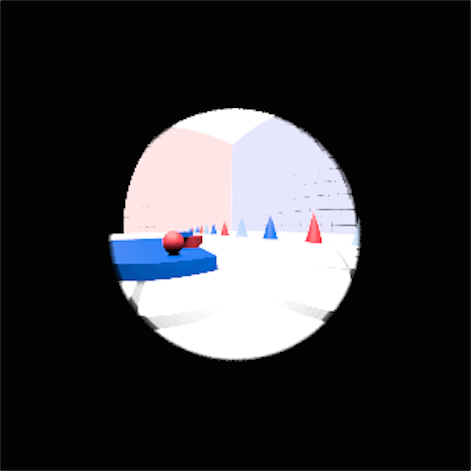
\includegraphics[width=40mm]{fisheye_screenshot.png}
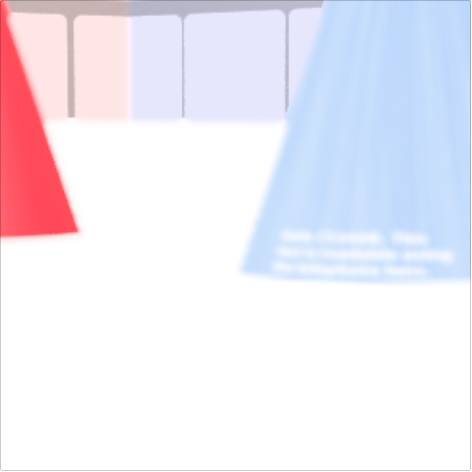
\includegraphics[width=40mm]{telephoto_screenshot.png}
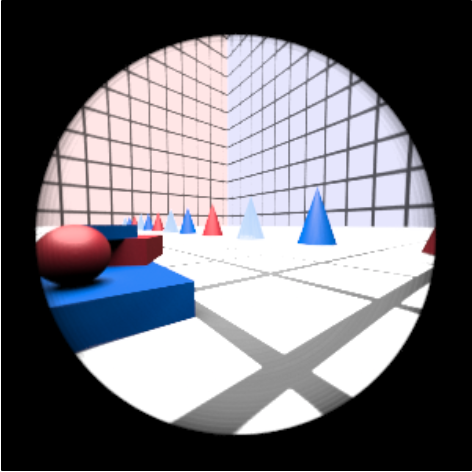
\includegraphics[width=40mm]{wide_screenshot.png}
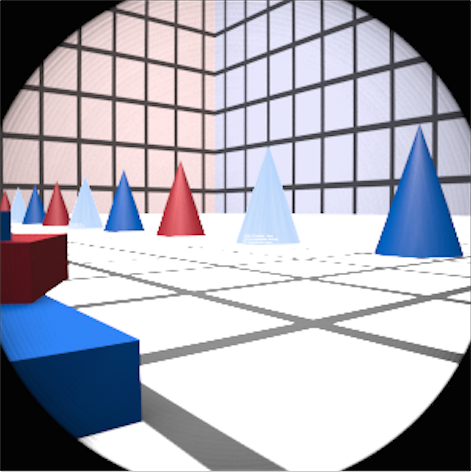
\includegraphics[width=40mm]{dgauss_screenshot.png}
\caption{Left to right: fisheye, telephoto, wide-angle, double gauss}
\end{figure}
\end{document}